\chapter{无人机视觉定位与堆体重建及体积测量测试与分析}
\label{cha:chap5}
\section{引言}
\label{sec:5.1}
做实验做实验做实验
\section{无人机视觉定位系统测试}
\label{sec:5.2}
\subsection{视觉定位系统实验步骤设计}
\label{sec:5.2.1}
在第二章,本文提出了一种结合二维码的SLAM视觉系统,利用该系统可以估计出带有真实尺度的相机位姿,以及能够得到真实世界坐标系下的
相机位置。本次实验主要利用上述方法在复杂封闭,且无GPS信号的环境下,结合二维码视觉标签进行无人机定位,通过获得到的位置信息信
息进行下一步的飞行控制。本次实验的准备过程主要分为三个步骤,布置场景,生成地图,无人机自主循迹。

首先是场景布置,选择在空旷场地中,布置二维码视觉标签,保证每个二维码的尺度大小完全一致,且二维码之间尽可能等间距布置,场景中的
二维码ID完全独立不同,设计图和实际布置图分别如图~\ref{fig:scene_imagine}和图~\ref{fig:scene_reality}所示。在本次实验中,所原选择的二维码实际大小为0.73m,相邻二维码之间的距
离为4m,整个实验区域面积为400$m^2$(20m*20m)。
\begin{figure}[H]
  \centering%
  \subcaptionbox{实验场景设计示意图\label{fig:scene_imagine}}{%    
    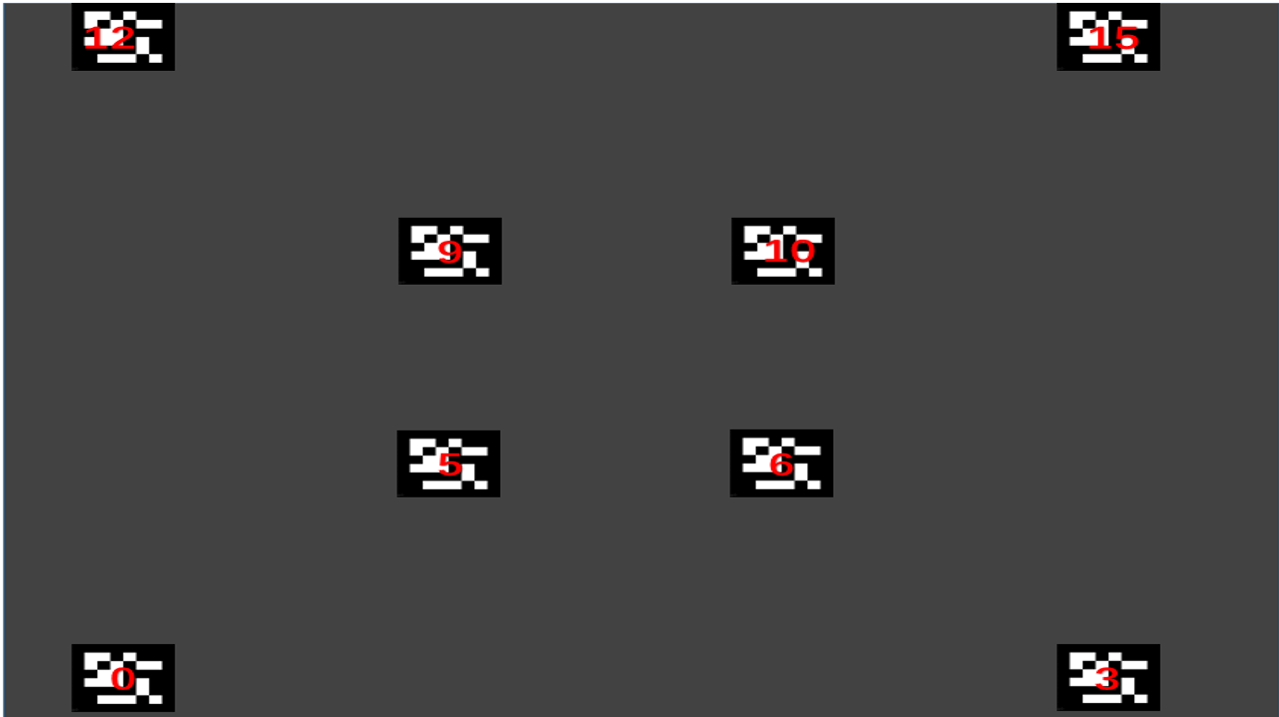
\includegraphics[height=6cm,width=6cm]{scene_imagine.png}}\hspace{4em}%
  \subcaptionbox{实验场景真实布置图\label{fig:scene_reality}}{%    
    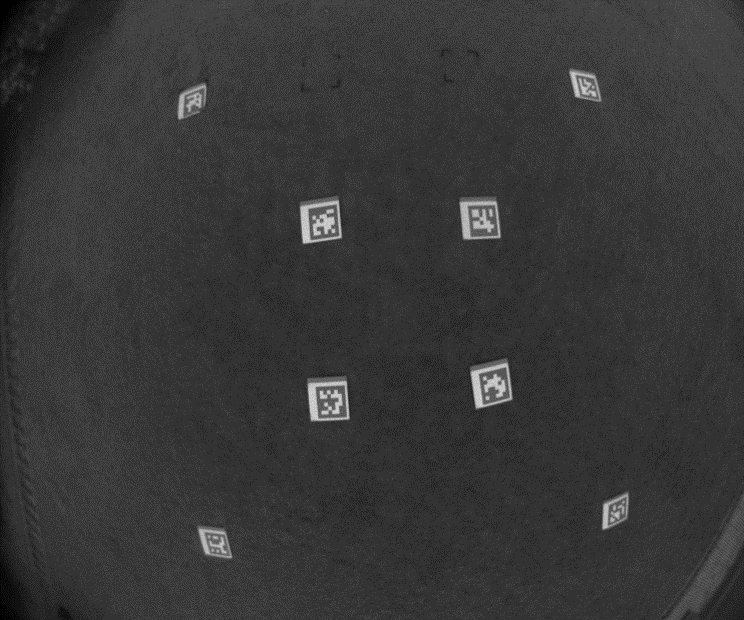
\includegraphics[height=6cm,width=6cm]{scene_reality.png}}
  \caption{实验场景示意图}
  \label{fig:scene}
\end{figure}

在布置好场景后,需要根据实际场景生成地图信息。当无人机首次在无先验地图的环境下飞行时,需要人工手动控制,完成无人机的飞行和地图
生成工作,在无人机的手动飞行过程中,其飞行区域需要尽可能覆盖所有场景以确保生产完整的地图,根据实际场景生成的地图如图~\ref{fig:map_generator}
所示,其中正方形框代表二维码,蓝色相机表示代表视觉定位产生的关键帧,点代表地图中的特征点。

\begin{figure}[H] % use float package if you want it here
  \centering
  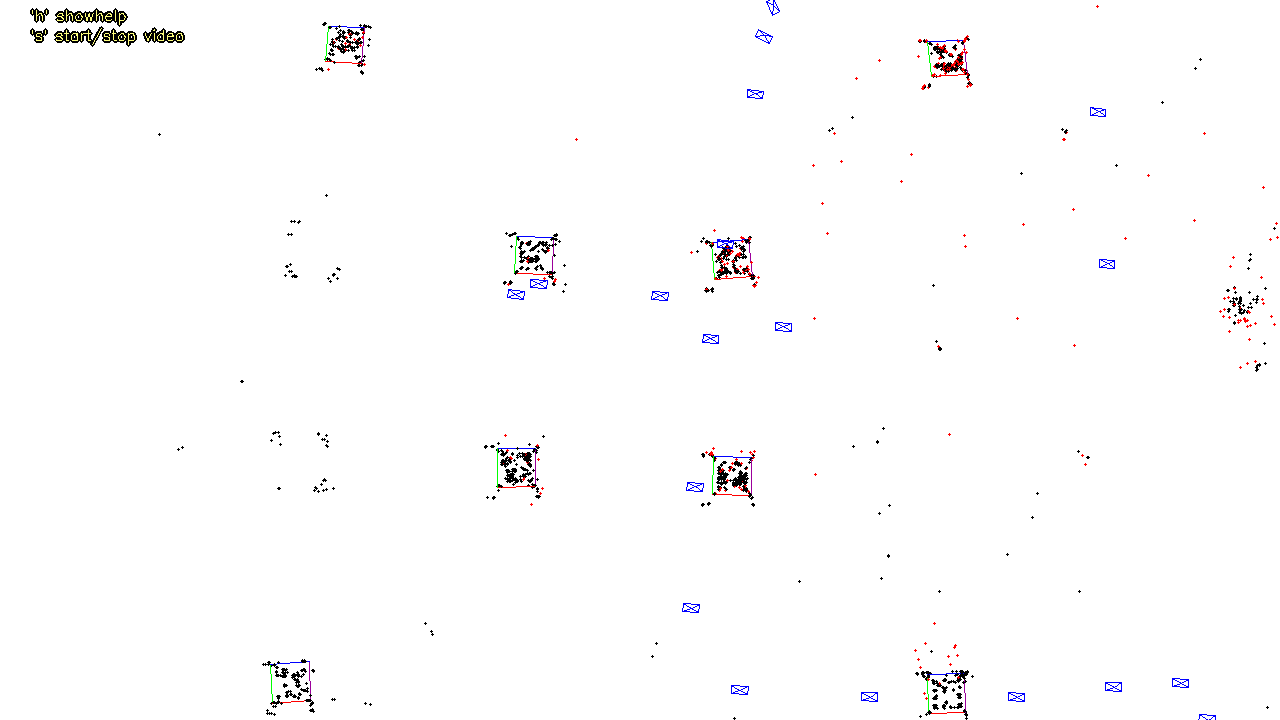
\includegraphics[height=8cm]{map_generator.png}
  \caption{视觉算法生成地图}
  \label{fig:map_generator}
\end{figure}

当获取到完整的地图信息地图后,可以让无人机按照认为规定的轨迹进行自动循迹飞行,首先设计如下图~\ref{fig:flight_route}所示的轨
迹图,其中起始点为ID=0的二维码处,红色箭头代表无人机的飞行轨迹,对于无人机的飞控过程,按照设定循迹点的方案来实现,即在整个轨迹
中给定多个循迹点坐标,使得无人机按照设定的坐标顺序进行飞行。
\begin{figure}[H] % use float package if you want it here
  \centering
  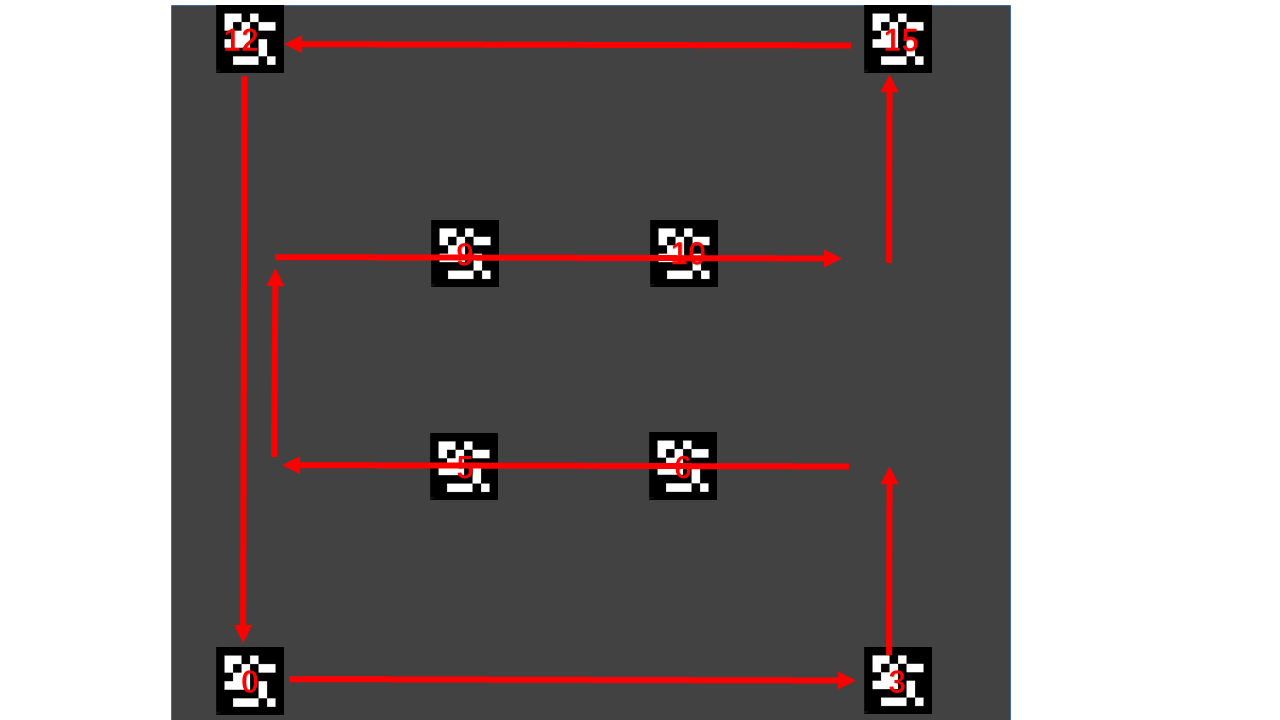
\includegraphics[height=8cm]{flight_route.png}
  \caption{无人机自主飞行轨迹设计图}
  \label{fig:flight_route}
\end{figure}
\subsection{视觉定位系统实验结果分析}
\label{sec:5.2.2}
按照上述实验流程让无人机进行自主飞行,可以直接获取到视觉算法生成的地图以及无人机在飞行的过程中生成的三维坐标,根据这些数据可以对
视觉算法关于无人机自主定位的效果进行定量的分析,本节主要从生成地图的精度,无人机三维坐标的精度以及轨迹精度三个方面进行定量分析。

首先对于地图精度,根据图~\ref{fig:scene_reality}生成的地图,通过对地图的解析,可以获取每一个二维码的三维位置坐标,如
表~\ref{tab:chap1:marker_pose}所示。

\begin{table}[h]
  \centering
  \caption{二维码标志位置实际测量值}
  \label{tab:chap1:marker_pose}
  \begin{tabular}{C{3.6cm}L{2.4cm}L{2.4cm}L{2.4cm}}
  \toprule
  \textbf{序号} & \textbf{X} & \textbf{Y} & \textbf{Z} \\
  \midrule
  0      & -2.63   & 	1.32 & 7 .86            \\
  3      & -14.69  & 	3.88 & 7.80            \\
  5      & -6.05 	 &  6.34 & 7.45           \\
  6      & -9.83 	 &  -9.83 & 7.45           \\
  9      & -5.13 	 &  10.44 & 7.30           \\
  10     & -9.17   &	11.22 &	7.24        \\
  12     & -0.33 	 &  13.56 & 7.34 	             \\
  15     & -12.25  & 	16.15 &	7.27            \\
  \bottomrule
  \end{tabular}
\end{table}

针对地图的精度,可以提出以下两个判断指标。\\
1)任意两个二维码之间距离的测量值和理论值的误差比较;\\
2)所有二维码是否在同一个坐标平面。

针对指标1,计算得到表~\ref{tab:chap1:marker_map_error},经过计算得到地图中二维码的误差精度为3.1$\%$。

\begin{table}[h]
    \centering
    \caption{二维码位置误差}
    \label{tab:chap1:marker_map_error}
    \begin{tabular}{C{1.6cm}C{1.6cm}C{2.4cm}C{2.4cm}C{3.2cm}}
    \toprule
    \textbf{ID1} & \textbf{ID2} & \textbf{实际值} & \textbf{理论值} & \textbf{误差率} \\
    \midrule
    0&	3&	12.33&	12&	2.75 $\%$\\
    0&	5&	6.07&	5.65&	7.43$\%$\\
    0&	6&	9.26&	8.94&	3.58$\%$\\
    0&	9&	9.46&	8.94&	5.82$\%$\\
    0&	10&	11.86&11.31&	4.86$\%$\\
    0&	12&	12.45&	12&	3.75$\%$\\
    0&  15&	17.67&	16.97&	4.12$\%$\\
    3&	5&	8.99&	8.94&	0.56$\%$\\
    3&	6&	5.85&	5.65&	3.54$\%$\\
    3&	9&	11.6&	11.31&	2.56$\%$\\
    3&	10&	9.18&	8.94&	2.68$\%$\\
    3&	12&	17.32&	16.97&	2.06$\%$\\
    3&	15&	12.51&	12&	4.25$\%$\\
    5&	6&	3.87&	4&	3.25$\%$\\
    5&	9&	4.21&	4&	5.25$\%$\\
    5&	10&	5.79&	5.65&	2.48$\%$\\
    5&	12&	9.21&	8.94&	3.02$\%$\\
    5&	15&	11.61&	11.31&	2.65$\%$\\
    6&	9&	5.75&	5.65&	1.77$\%$\\
    6&	10&	4.13&	4&	3.25$\%$\\
    6&	12&	11.47&	11.31&	1.41$\%$\\
    6&	15&	9.33&	8.94&	4.36$\%$\\
    9&	10&	4.11&	4&	2.75$\%$\\
    9&	12&	5.72&	5.65&	1.24$\%$\\
    9&	15&	9.12&	8.94&	2.01$\%$\\
    10&	12&	9.15&	8.94&	2.35$\%$\\
    10&	15&	5.81&	5.65&	2.83$\%$\\
    12&	15&	12.2&	12&	1.67$\%$\\  
    \bottomrule
    \end{tabular}
\end{table}

针对指标2,绘制出每个二维码的在同一个坐标平面的误差情况,如图~\ref{fig:marker_map_error_Z}所示,平均误差为0.18m,
可以认定所有二维码基本都在同一水平面内。
\begin{figure}[H] % use float package if you want it here
  \centering
  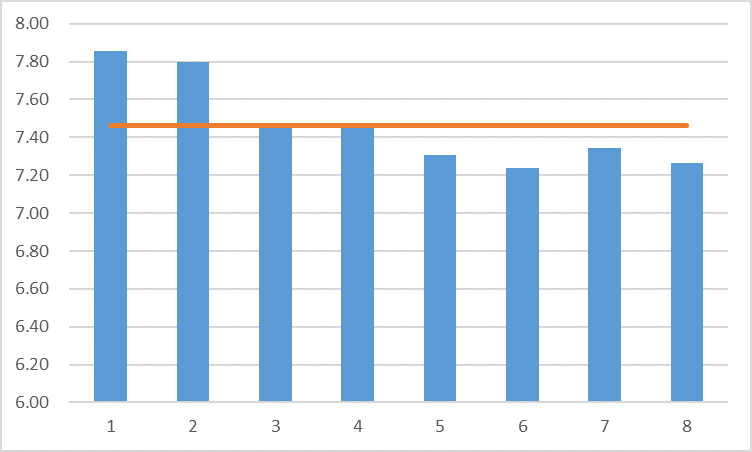
\includegraphics[height=8cm]{marker_map_error_Z.png}
  \caption{二维码Z方向数据}
  \label{fig:marker_map_error_Z}
\end{figure}
其次对于无人机三维坐标的精度,以无人机自带GPS测距仪器测定出的坐标为真值,和视觉算法计算出来的位置信息进行对比,选择无人机
在0-800帧的数据,在X、Y、Z方向得到的结果分别如图~\ref{fig:chap2:pose_xyz}所示,其中蓝色连线为视觉算法检测出的坐标值,红色
连线无人机GPS检测出的真实值。
\begin{figure}[h]
  \centering
    \subcaptionbox{X方向GPS和视觉算法对比图}{\label{fig:chap1:pose_x}
    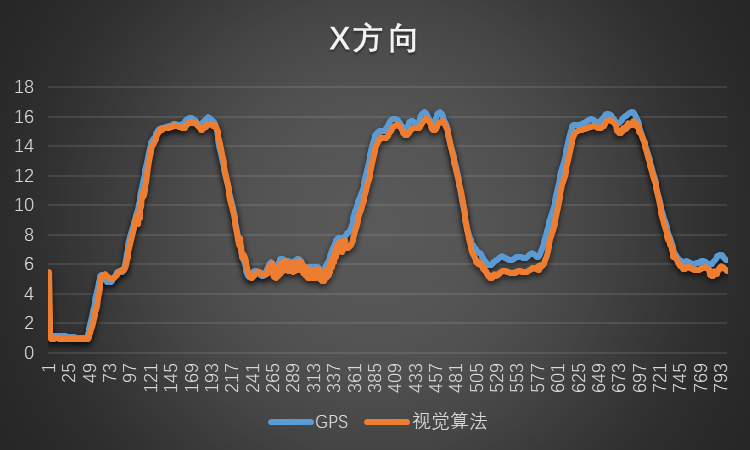
\includegraphics[width=6cm]{pose_x.png}\hskip2cm}
    \subcaptionbox{Y方向GPS和视觉算法对比图}{\label{fig:chap1:pose_y}
    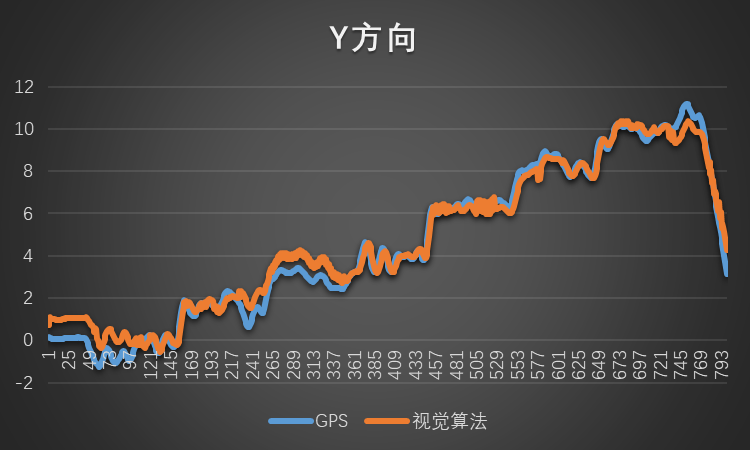
\includegraphics[width=6cm]{pose_y.png}}
  \vskip0.5cm
    \subcaptionbox{Z方向GPS和视觉算法对比图}{\label{fig:chap1:pose_z}
    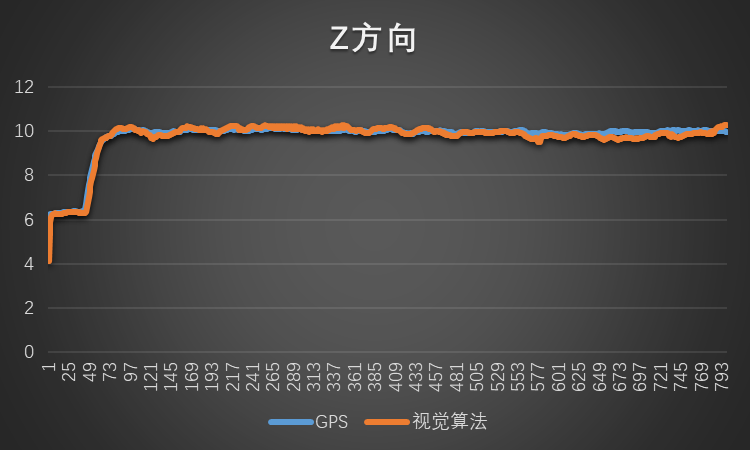
\includegraphics[width=6cm]{pose_z.png}\hskip2cm}
  \caption{各方向GPS和视觉算法对比图}\label{fig:chap2:pose_xyz}
\end{figure}
随后,计算真值和测量值之间的误差,在X、Y、Z方向分别得到结果如图~\ref{fig:chap2:pose_error_xyz}所示,对于X、Y、Z三个方向分别可以
得到距离误差为0.22m、0.37m、0.107m。
\begin{figure}[H]
    \centering
      \subcaptionbox{X方向GPS和视觉算法对比图}{\label{fig:chap1:pose_error_x}
      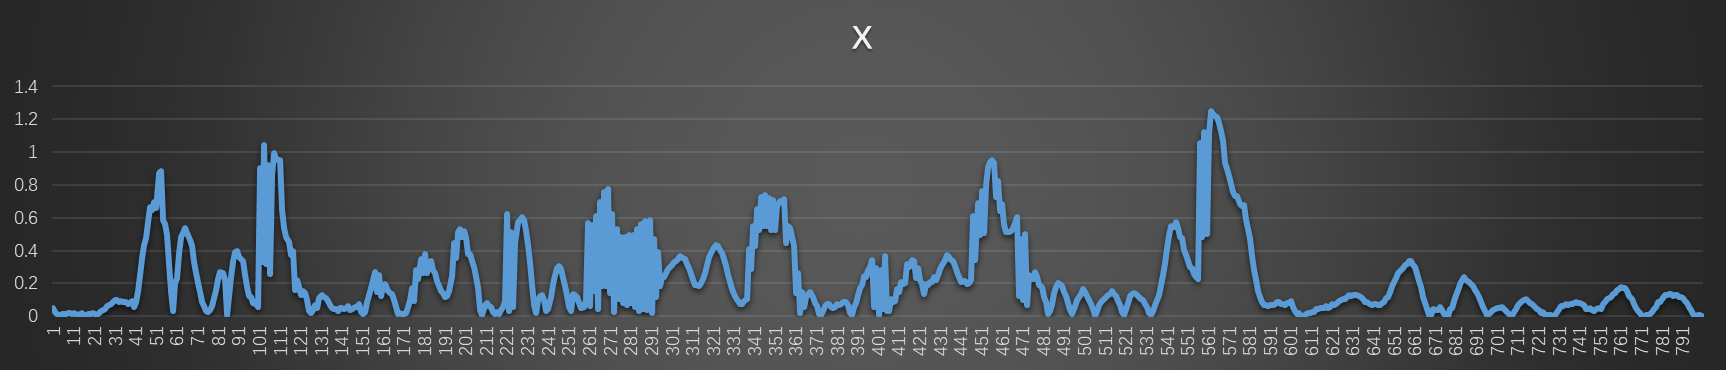
\includegraphics[width=12cm]{pose_error_x.png}}
    \vskip0.5cm
      \subcaptionbox{Z方向GPS和视觉算法对比图}{\label{fig:chap1:pose_error_y}
      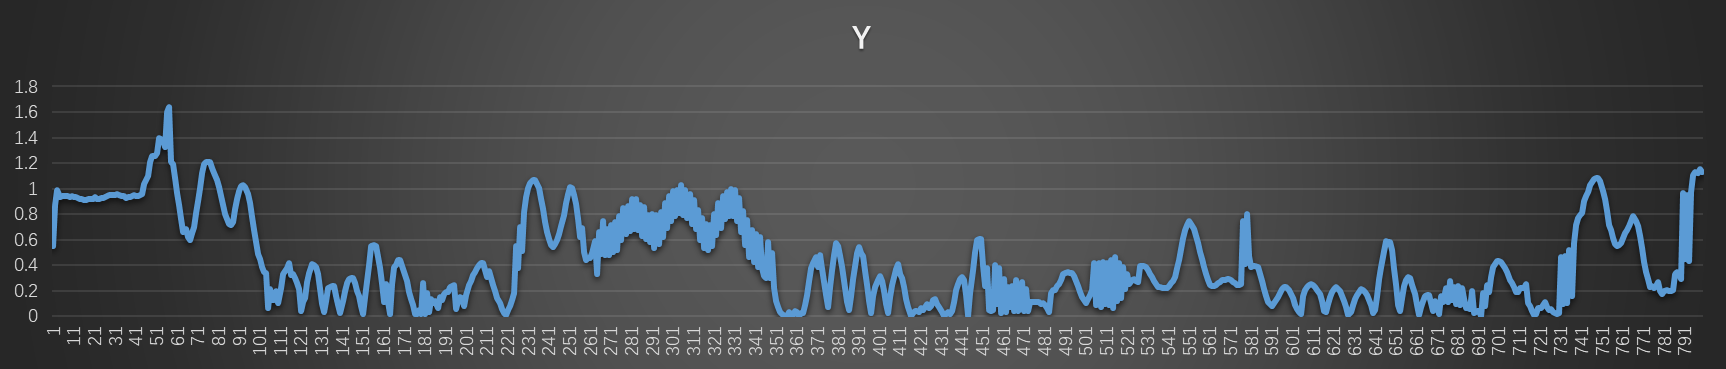
\includegraphics[width=12cm]{pose_error_y.png}}
    \vskip0.5cm
      \subcaptionbox{Z方向GPS和视觉算法对比图}{\label{fig:chap1:pose_error_z}
      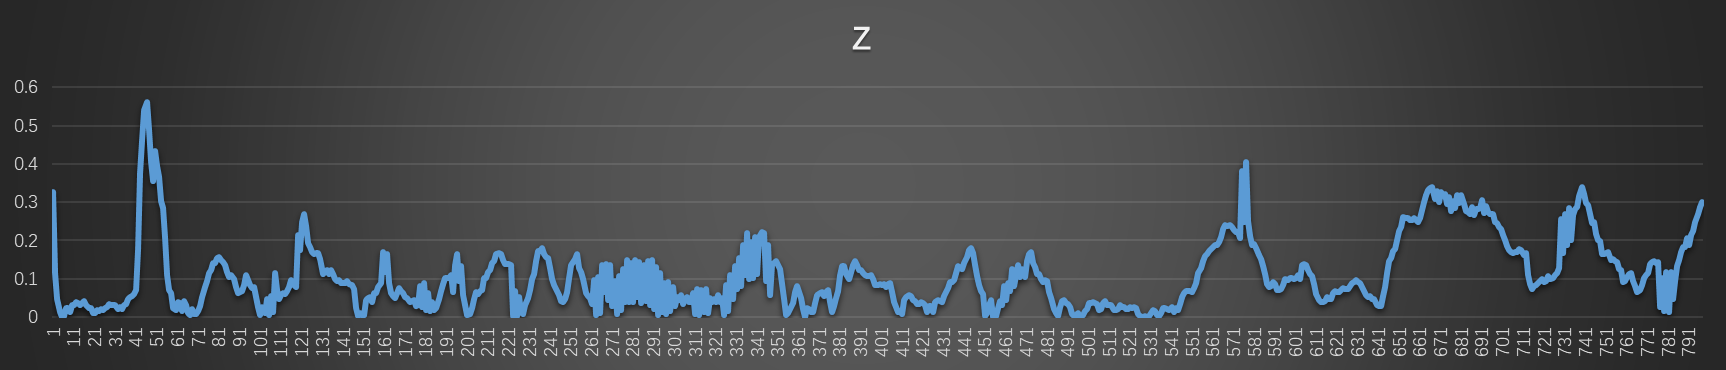
\includegraphics[width=12cm]{pose_error_z.png}}
    \caption{各方向GPS和视觉算法误差对比图}\label{fig:chap2:pose_error_xyz}
\end{figure}
最后,对无人机的轨迹精度进行对比。无人机在自主飞行过程中能够产生实时的相对于真实世界坐标系的定位信息,将其与GPS生成的定位信息
进行对比,如图~\ref{fig:pose_map}所示。
\begin{figure}[H] % use float package if you want it here
  \centering
  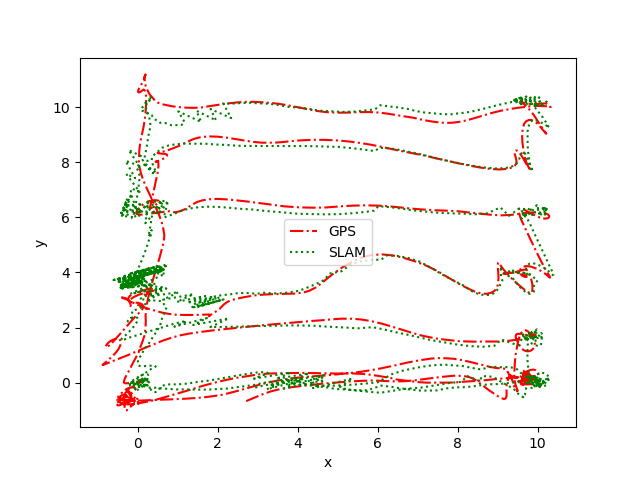
\includegraphics[height=10cm]{pose_map.png}
  \caption{无人机轨迹对比示意图}
  \label{fig:pose_map}
\end{figure}
对于无人机的直飞路线,误差较小,GPS和视觉算法测算出的轨迹基本吻合,但是在对于转弯改变方向的区间,两者之间的相对误差则较大,考虑
其原因为在转弯处所设计的循迹点相对比较稠密,导致在该区域内无人机需要改变的方向更大,导致视觉算法在测算时由于方法振动的缘故产生
较大的误差。





\section{三维重建系统测试}
\label{sec:5.3}
在本文~\ref{sec:3.2.3}节中,提出了三维重建存在的一些问题,包括对场景进行三维重建时,匹配耗时严重和点云准确性较低,甚至无法重建出三维点云,
本实验将结合~\ref{sec:3.3}节提出的方法对三维重建进行改进。
\subsection{匹配实效性测试}
通过~\ref{sec:3.3.2}节对输入图像匹配模式的分析,本实验共选择150张图像(图片选择过少的话,各匹配模式之间的耗时差异会过小)作为输入图片,每
张图像的大小为960*544。各匹配模式包括完全匹配,序列匹配,空间匹配,传递匹配和自定义匹配,对于空间匹配,在对室内堆体三维重建时,难以获取准确的空间位置信息,本实验将排除该匹配方式的对比
其中自定义匹配以实时运行的SLAM匹配信息作为匹配结果。SLAM处理代码如~\ref{code:SLAM_process}下:
\begin{lstlisting}[
  language=C++,
  numbers=left,                
  numberstyle=\footnotesize,
  frame=single,     
  basicstyle=\small\tt,    
  escapeinside = '',
  caption={SLAM处理数据集~C++~实现},
  label={code:SLAM_process}]
'//SLAM处理数据集'

if (mpCurrentKeyFrame->mnId > 4)
  {

   std::vector<KeyFrame*> cos = 
    mpCurrentKeyFrame->GetBestCovisibilityKeyFrames(covisibleNum);
   cv::Mat rotation = mpCurrentKeyFrame->GetRotation();
   cv::Mat translation = mpCurrentKeyFrame->GetTranslation();

   Eigen::Matrix3d r2 = Converter::toMatrix3d(rotation);
   Eigen::Quaterniond q2(r2);

   fs1 << mpCurrentKeyFrame->mnFrameId << ",";
   for (int k = 0; k < cos.size(); k++)
   {
    fs1 << cos[k]->mnFrameId << ",";
   }

   fs1 << "|" << 
   q2.w() <<","<< q2.x() <<","<< q2.y() <<","<< q2.z() <<","
   << translation.at<float>(0) <<","
   << translation.at<float>(1) <<","
   << translation.at<float>(2) 
   << std::endl;
  }

\end{lstlisting}

对任意一帧图像,在SLAM处理后只处理并保存关联关键帧大于4帧的图像,依次获取与该帧匹配度最高的4帧和该帧所对应的位
姿(R,t)结果如表~\ref{tab:SLAM_result}所示。

\begin{table}[h]
  \centering
  \caption{SLAM处理结果}
  \label{tab:SLAM_result}
  \begin{tabular}{C{1.2cm}C{4.0cm}C{8.6cm}}
  \toprule
  \textbf{当前帧} & \textbf{匹配帧集合} &\textbf{位姿}  \\
  \midrule
  4&[5 3 2 1 ]&[R:0.989 -0.008 -0.137 0.053 t:-0.00 0.017 -0.033]\\
  3&[4 5 2 1 ]&[R:0.989 -0.031 -0.163 0.056 t:-0.001 0.015 -0.030]\\
  6&[5 7 4 8 ]&[R:0.987 -0.019 -0.131 0.090 t:-0.018 0.016 -0.064]\\
  2&[3 4 5 1 ]&[R:0.981 -0.018 -0.184 0.057 t:0.000 0.015 -0.025]\\
  8&[9 7 10 6 ]&[R:0.989 -0.039 -0.111 0.079 t:-0.034 0.014 -0.104]\\
  $\dots$   &   $\dots$ &   $\dots$\\
  $\dots$   &   $\dots$ &   $\dots$\\
  $\dots$   &   $\dots$ &   $\dots$\\
  $\dots$   &   $\dots$ &   $\dots$\\
  145&[147 146 148 149 ]&[R:0.978 -0.118 -0.148 0.083 t:0.026 0.030 0.117]\\
  149&[148 147 146 145 ]&[R:0.983 -0.109 -0.114 0.083 t:0.0123 0.020 0.033]\\
  146&[147 148 145 149 ]&[R:0.972 -0.148 -0.168 0.067 t:0.017 0.0334 0.099]\\
  151&[4 5 152 3 ]&[R:0.989 -0.096 -0.099 0.047 t:0.001 0.010 -0.057]\\
  154&[12 13 11 10 ]&[R:0.992 -0.080 -0.085 0.021 t:-0.030 0.004 -0.204]\\
  \bottomrule
  \end{tabular}
\end{table}

各个匹配模式之间的耗时情况和匹配准确度如表~\ref{tab:match_compare}所示。
\begin{table}[h]
  \centering
  \caption{各匹配模式耗时与精度情况对比表}
  \label{tab:match_compare}
  \begin{tabular}{C{3.6cm}C{2.4cm}L{2.4cm}L{2.4cm}C{3.6cm}}
  \toprule
  \textbf{匹配模式} & \textbf{耗时(/s)} &\textbf{匹配精度}  \\
  \midrule
  完全匹配  &504& 精度较高\\
  序列匹配  &94&精度较高\\
  传递匹配  &7 &精度较差\\
  自定义匹配  &实时得到结果 &精度高\\
  \bottomrule
  \end{tabular}
\end{table}



\subsection{点云精度测试}
在面对部分重复度高,表面问题贫瘠的场景中,三维重建往往难以生成有效的点云,按照第节提出的方法可以以SLAM生成的keyFrame Database
作为先验知识来改善三维重建的结果。本实验考虑到地下车库场景重复度高,且存在反光现象,选择了地下车库作为实验场景,按照环形有闭环的
路径采集了一系列图像,部分图像如~\ref{test_3D_garage}所示。
如图~\ref{fig:test_3D_garage}所示
\begin{figure}[H] % use float package if you want it here
  \centering
  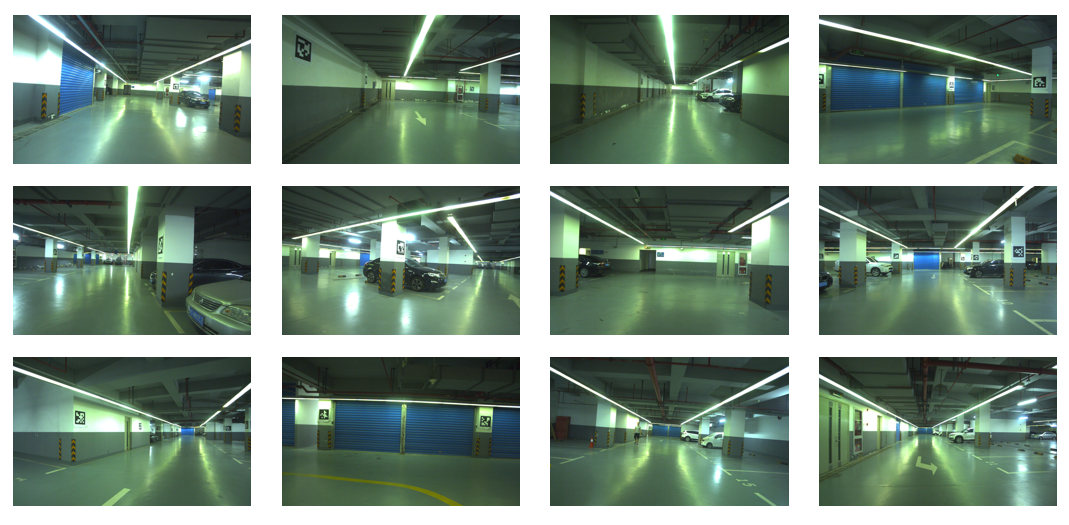
\includegraphics[height=6cm,width=9.7cm]{test_3D_garage.png}
  \caption{地下车库环形图像}
  \label{fig:test_3D_garage}
  \end{figure}
对于普通三维重建方法而言,地下车库场景重建场景点云难度较大,因为场景中的场景重复度高,匹配精度较低,且反光场景的加入又会导致相机
的位姿估计出现偏差,三维重建无法生成有效的点云结果,如图~\ref{fig:test_3D_badresult}所示。因此需要结合SLAM的结果来作为三维
重建的先验知识,可以重建出较好的结果,结果如图~\ref{fig:test_3D_goodresult}所示。
  \begin{figure}[h]
  \centering
    \subcaptionbox{结合SLAM三维重建}{\label{fig:test_3D_goodresult}
    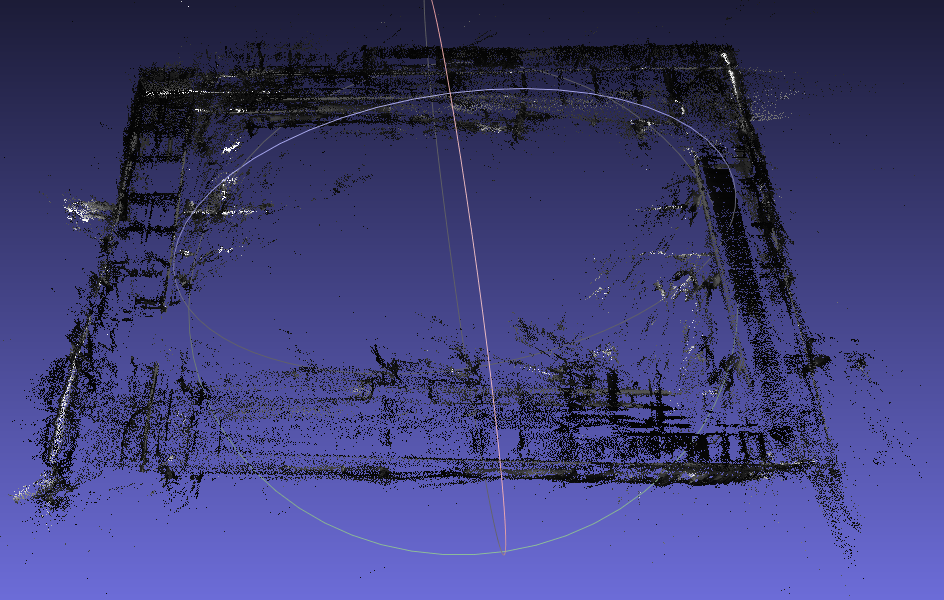
\includegraphics[height=6cm,width=9.7cm]{test_3D_goodresult.png}}
  \vskip0.5cm
    \subcaptionbox{直接三维重建}{\label{fig:test_3D_badresult}
    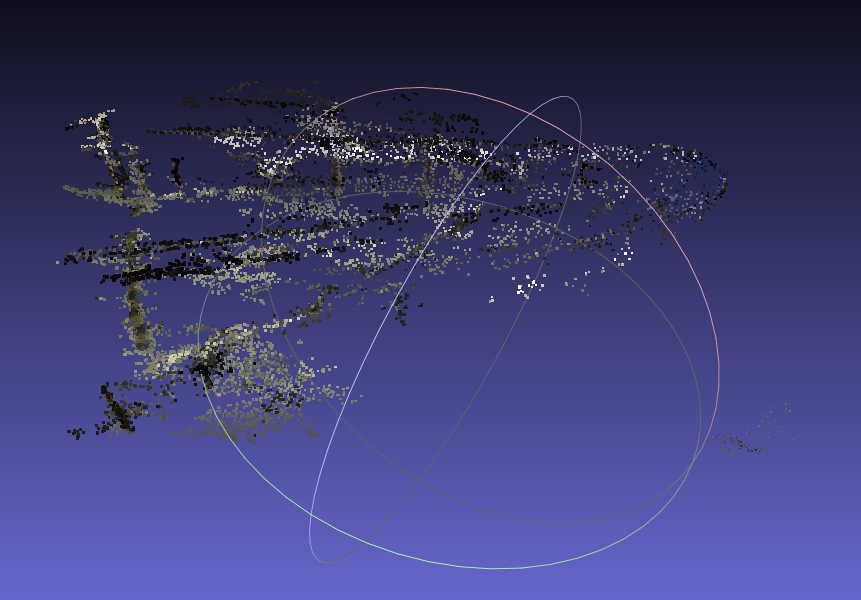
\includegraphics[height=6cm,width=9.7cm]{test_3D_badresult.png}}
  \caption{地下车库三维重建对比图}\label{fig:test_3D}
\end{figure}

\section{堆体体积测量系统测试}
\label{sec:5.4}
在第四章,本文提出了一种基于纯视觉方法来测算场景中物体体积的方法,基于对实验场景进行的三维重建结果,整个实验步骤主要包括以下
四个方面1)解析水平面方程2)估计场景实际尺度3)点云提纯4)计算三维点云的体积。在对测算场景体积之前,需要收集该场景的连续视频
帧以获取其三维重建的结果,考虑到稠密点云的点集数量过大,在遍历和查询时都会比较耗时,且稀疏点云也包含了每个特征点的坐标信息和
相机的位姿信息,后续在解析水平面方程和估计场景实际尺度时选择稀疏点云作为分析对象。
\subsection{解析水平面方程}
\label{sec:5.4.1}
1.	场景布置:在待测场景中需要布置多个不同的Aruco二维码,一方面提高场景三维重
建的稳定性和准确性,另外进一步为后续水平面方程的解析提供数据。在布置场景时,需要注意两个问题:1)若所布置的所有Aruco二维码的
所有下边沿都位于同一条直线上; 2)应该尽可能将所有Aruco的二维码的下边沿都与待求水平面贴合,以保证水平面方程求解的准确性,若
无法实现水平面的贴合要求,则需要进一步保证所有下边沿都位于同一水平面上,那么对计算得到的水平面进行空间变换即可得到真实水平面
方程。

2.	数据收集:可以通过单目相机对场景进行连续采集,在采集视频的过程中需要保证大部分视频帧中都能够采集到完成的二维码,所有的采
集结果如图~\ref{fig:getVolume_inputCamera}所示。

\begin{figure}[H] % use float package if you want it here
  \centering
  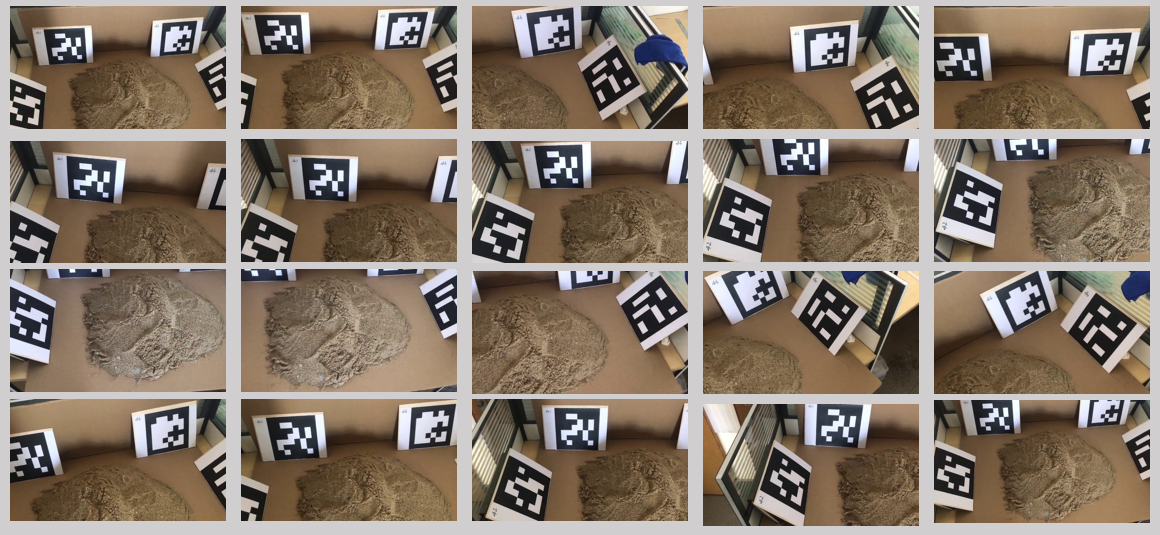
\includegraphics[height=6cm]{getVolume_inputCamera_1.png}
  \caption{三维重建输入视频序列图}
  \label{fig:getVolume_inputCamera}
  \end{figure}

3.	三维重建:可以直接将上述这些包含二维码的视频帧序列作为三维重建的输入以获取场景的点云,重建的结果如图
~\ref{fig:getVolume_3dconstr_noplane}所示。
\begin{figure}[H] % use float package if you want it here
  \centering
  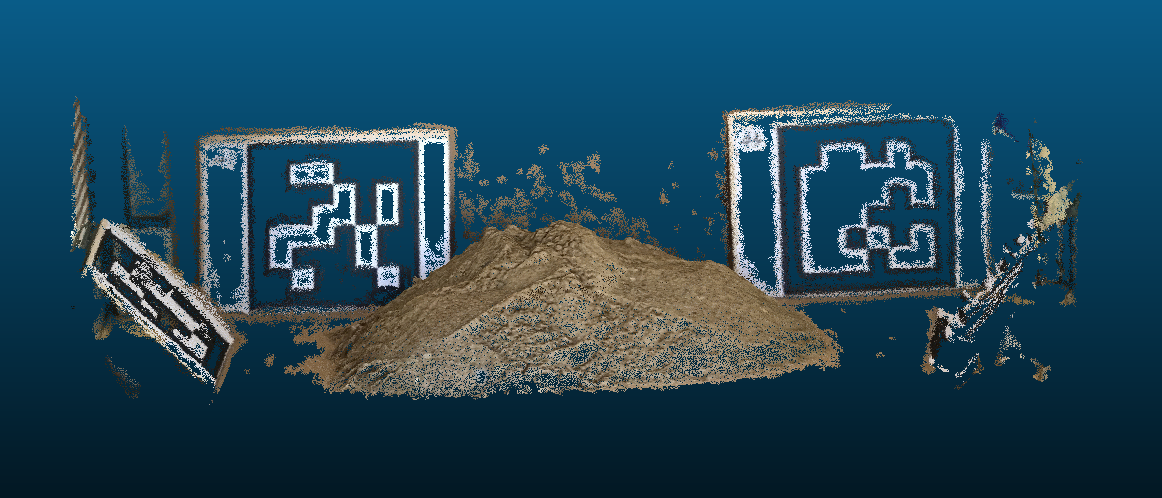
\includegraphics[height=6cm]{getVolume_3dconstr_noplane_1.png}
  \caption{三维重建点云结果示意图}
  \label{fig:getVolume_3dconstr_noplane}
  \end{figure}

4.	按照4.2.1和4.2.2小节的方式获取2D图像中的角点坐标和对应的三维重建的3D坐标,部分对应关系如
表~\ref{tab:chap1:2D_3D}所示。其中最近的2D坐标代表通过三维重建获进行特征点提取时的最近坐标,
当3D为-1时,则代表三维重建中的点云没有和该2D图像相对应的3D点。

\begin{table}[h]
  \centering
  \caption{2D坐标和3D坐标关系对应表}
  \label{tab:chap1:2D_3D}
  \begin{tabular}{C{1.6cm}L{2.4cm}L{4.4cm}L{4.4cm}}
  \toprule
  \textbf{图像名称} & \textbf{2D坐标} &\textbf{最近点2D坐标} &  \textbf{3D坐标}  \\
  \midrule
  1613.jpg  &[724, 344]   &[720.478,  343.642]  & -1\\
            &[512, 338]   &[514.977,  337.341]  & [1.75459, -1.35326, 8.97379]\\
  1641.jpg  &[901, 327]   &[902.283,  326.125]  & [3.75985, -1.35022, 8.76246]\\
            &[691, 305]   &[686.783,  313.456]  & [1.74998, -1.29991, 8.97196]\\
  1631.jpg  &[822, 342]   &[825.233,  345.432]  &[3.75985, -1.35022, 8.76246]\\
            &[615, 324]   &[607.253,  323.576]  &[1.69161, -1.38207, 8.97119]\\
  1561.jpg  &[652, 277]   &[649.351,  274.972]  &[3.75985, -1.35022, 8.76246]\\
            &[453, 298]   &[455.467,  297.046]  &[1.75459, -1.35326, 8.97379]\\
  1897.jpg  &[775, 283]   &[775.325,  282.267]  &[3.75985, -1.35022, 8.76246]\\
            &[607, 276]   &[607.673,  276.95]   &[1.75459, -1.35326, 8.97379]\\
  1897.jpg  &[457, 270]   &[461.465,  266.988]  & -1\\
            &[295, 267]   &[296.426,  266.952]  &[-2.24158, -1.3894, 9.26188]\\
  1911.jpg  &[783, 278]   &[780.128,  273.717]  &[3.75985, -1.35022, 8.76246]\\
            &[615, 272]   &[615.711,  273.065]  &[1.75459, -1.35326, 8.97379]\\
  1911.jpg  &[464, 267]   &[463.551,  266.358]  &-1\\
            &[302, 265]   &[303.311,  263.918]  &[-2.24158, -1.3894, 9.26188]\\
  \bottomrule
  \end{tabular}
\end{table}

5.	添加方程:根据4.2.3小节提出的方法,通过上述三维点可以计算出平面方程的参数,可以在原本缺失水平面的点云中按照解析方程添加
点云即可,结果如图~\ref{fig:getVolume_3dconstr}所示,其中红色点云即为水平面。
\begin{figure}[H] % use float package if you want it here
  \centering
  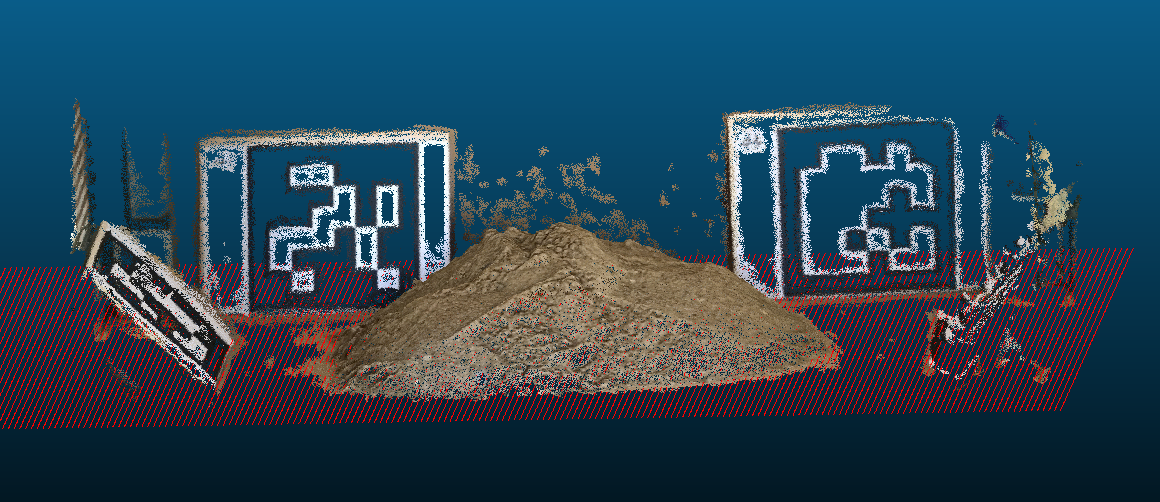
\includegraphics[height=6cm]{getVolume_3dconstr_1.png}
  \caption{三维重建输入视频序列图}
  \label{fig:getVolume_3dconstr}
  \end{figure}

\subsection{估计堆体实际尺度}
\label{sec:5.4.2}
1.	获取绝对尺度:根据图~\ref{fig:getVolume_Kabs}所示,分别可以获得在ID = 43的二维码坐标系下的相机位姿,如表~\ref{tab:chap1:2D_3D}
前两行,可以计算出在这两帧之间相机移动的绝对距离为0.464m。
\begin{figure}[H] % use float package if you want it here
  \centering
  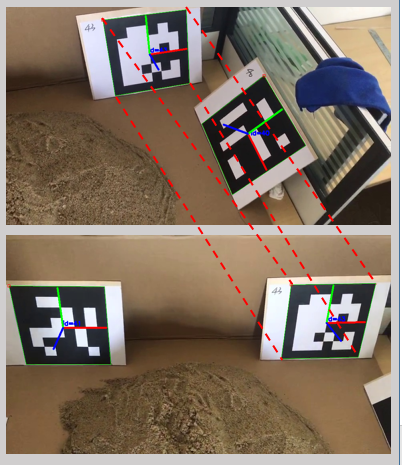
\includegraphics[height=8cm]{getVolume_Kabs.png}
  \caption{绝对尺度}
  \label{fig:getVolume_Kabs}
  \end{figure}
2.	获取相对尺度:从三维重建的结果中提取出这两帧在参考坐标系下的相机位姿,如表~\ref{tab:chap1:2D_3D}后两行,可以计算出这在这两帧之
间相机移动的相对距离为4.924。
\begin{table}[h]
  \centering
  \caption{2D坐标和3D坐标关系对应表}
  \label{tab:chap1:2D_3D}
  \begin{tabular}{C{3.6cm}L{2.4cm}L{2.4cm}L{2.4cm}C{3.6cm}}
  \toprule
  \textbf{序号} & \textbf{$T_x$} &\textbf{$T_y$} &  \textbf{$T_z$} &  \textbf{距离} \\
  \midrule
  1027.jpg  &-0.127325& -0.172455& 0.980864& \\
  1167.jpg  &0.324499 &-0.0655995& 0.969803&0.464\\
  1027.jpg  &-6.06873 &1.87705   & -2.13389&         \\
  1167.jpg  &-1.20871 &2.09888   & -1.37369&4.924 \\
  \bottomrule
  \end{tabular}
\end{table}

3.	估计尺度:按照公式~\ref{equ:getVolume_K}可以简略估计出该煤堆场景实际大小和三维重建结果的尺度大小之间的尺因子
K = 10.61。
\subsection{堆体体积估计}
针对体积测量实验,本文拟采用如下方式验证所提方法是否能够测量出堆体体积,以及是否满足精度要求:首先使用测量仪器检测出待测堆体
的实际体积真值,随后将堆体分别摆放成单个堆体,两个堆体,三个堆体的形式,按照第~\ref{cha:chap4}章的流程,检测三次实验是否和
真值之间的误差衡量视觉算法的精确度,以及三次测量值之间的数值比较,衡量视觉算法测量的稳定性。具体步骤如下:\\
1. 将某一堆体放置在水平面上,并在堆体周围放置5个二维码以估计尺度和水平面方程。\\
2. 对上述场景以视频的形式进行图像采集,提取视频中的图像,将数据集的数量控制在200张左右,且每张图像的分辨率在50万左右。\\
3. 对上述采集到的图像进行二维码检测与识别,记录下每张图像中的二维码ID以及角点坐标。。\\
4. 对上述采集到的图像进行稀疏重建,记录下稀疏点云中的3D点和每张图像角点之间的映射关系。\\
5. 按照~\ref{sec:4.2}估计堆体出水平面方程。\\
6. 按照~\ref{sec:4.3}估计出堆体的尺度大小。\\
7. 对稀疏点云进行稠密重建,并将所求解出的水平面方程添加至稠密点云中。\\
8. 按照~\ref{sec:4.4}估计出当前堆体的体积大小。\\
9. 将单个堆体分别设计成2个堆体和3个堆体的情况,重复步骤2$~$8,计算不同场景对应的体积。\\
10 根据结果定量分析上述视觉算法测量堆体的准确性和稳定性。

结果如表~\ref{tab:volume_test_1}$\textasciitilde$~\ref{tab:volume_test_3}所示。
\begin{table}[htb]
  \centering
  \caption{体积测量结果-\uppercase\expandafter{\romannumeral1}}
  \label{tab:volume_test_1}
  \begin{tabular}{C{2.4cm}C{2.0cm}C{8.0cm}C{2cm}}
  \toprule
  \textbf{实验批次} & \textbf{图像集数量} & \textbf{堆体场景预览} & \textbf{图像分辨率} \\
  \midrule
  1 & 186   & 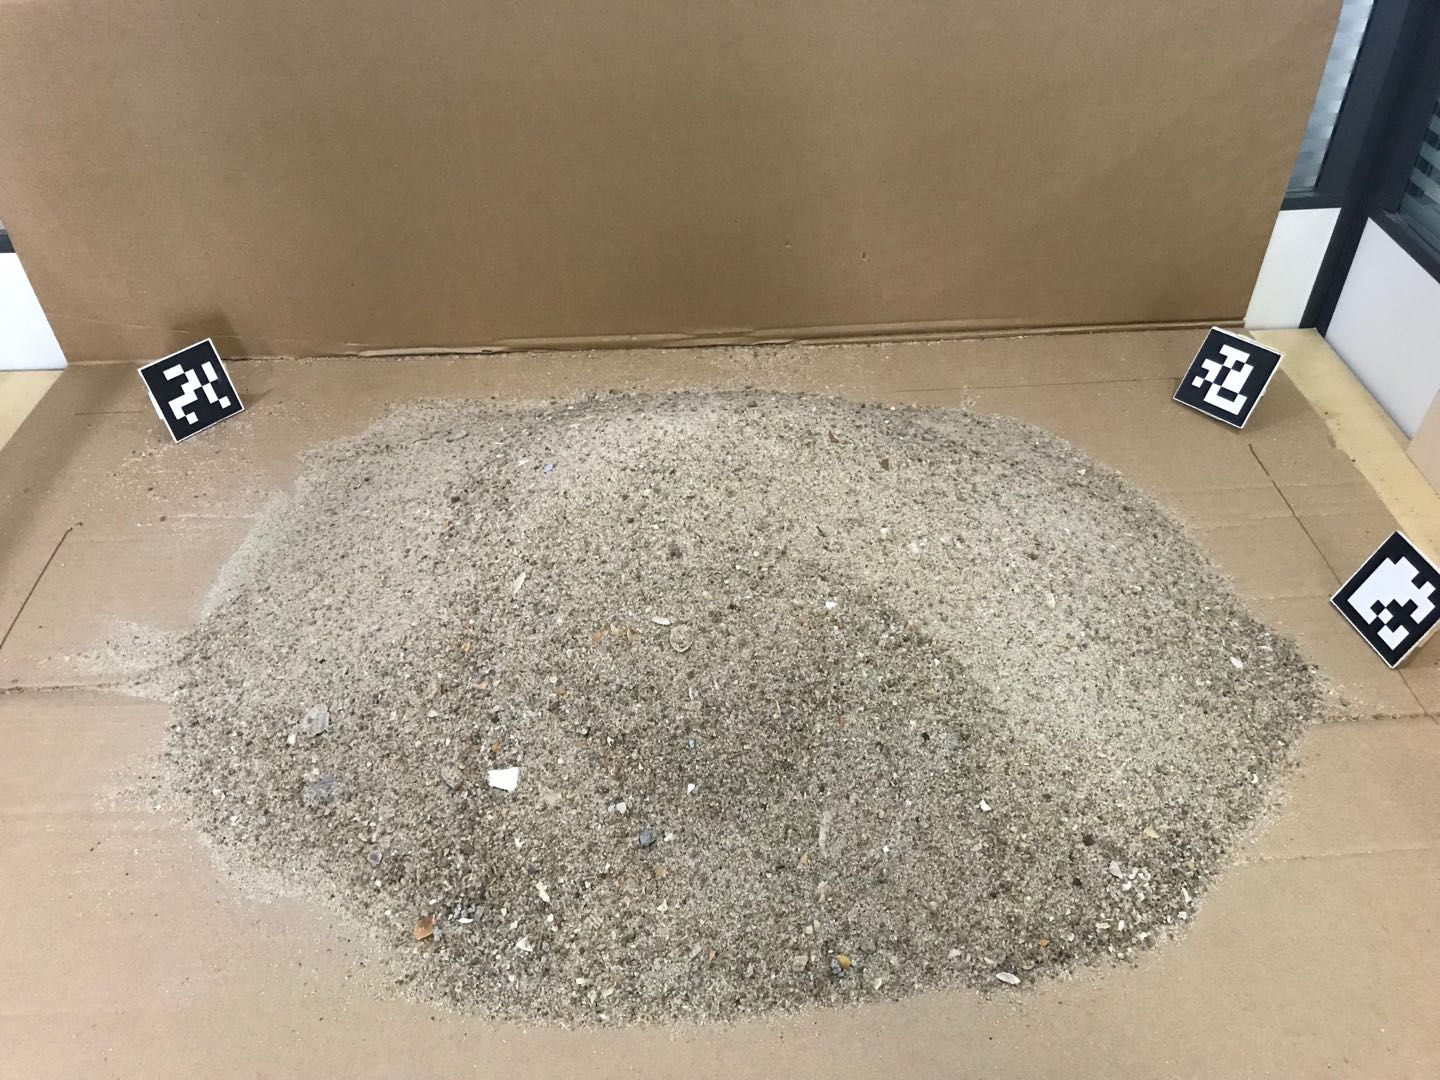
\includegraphics[width=7.5cm, height=5cm]{test_1.png} & 960*455 \\
  2 & 201   & 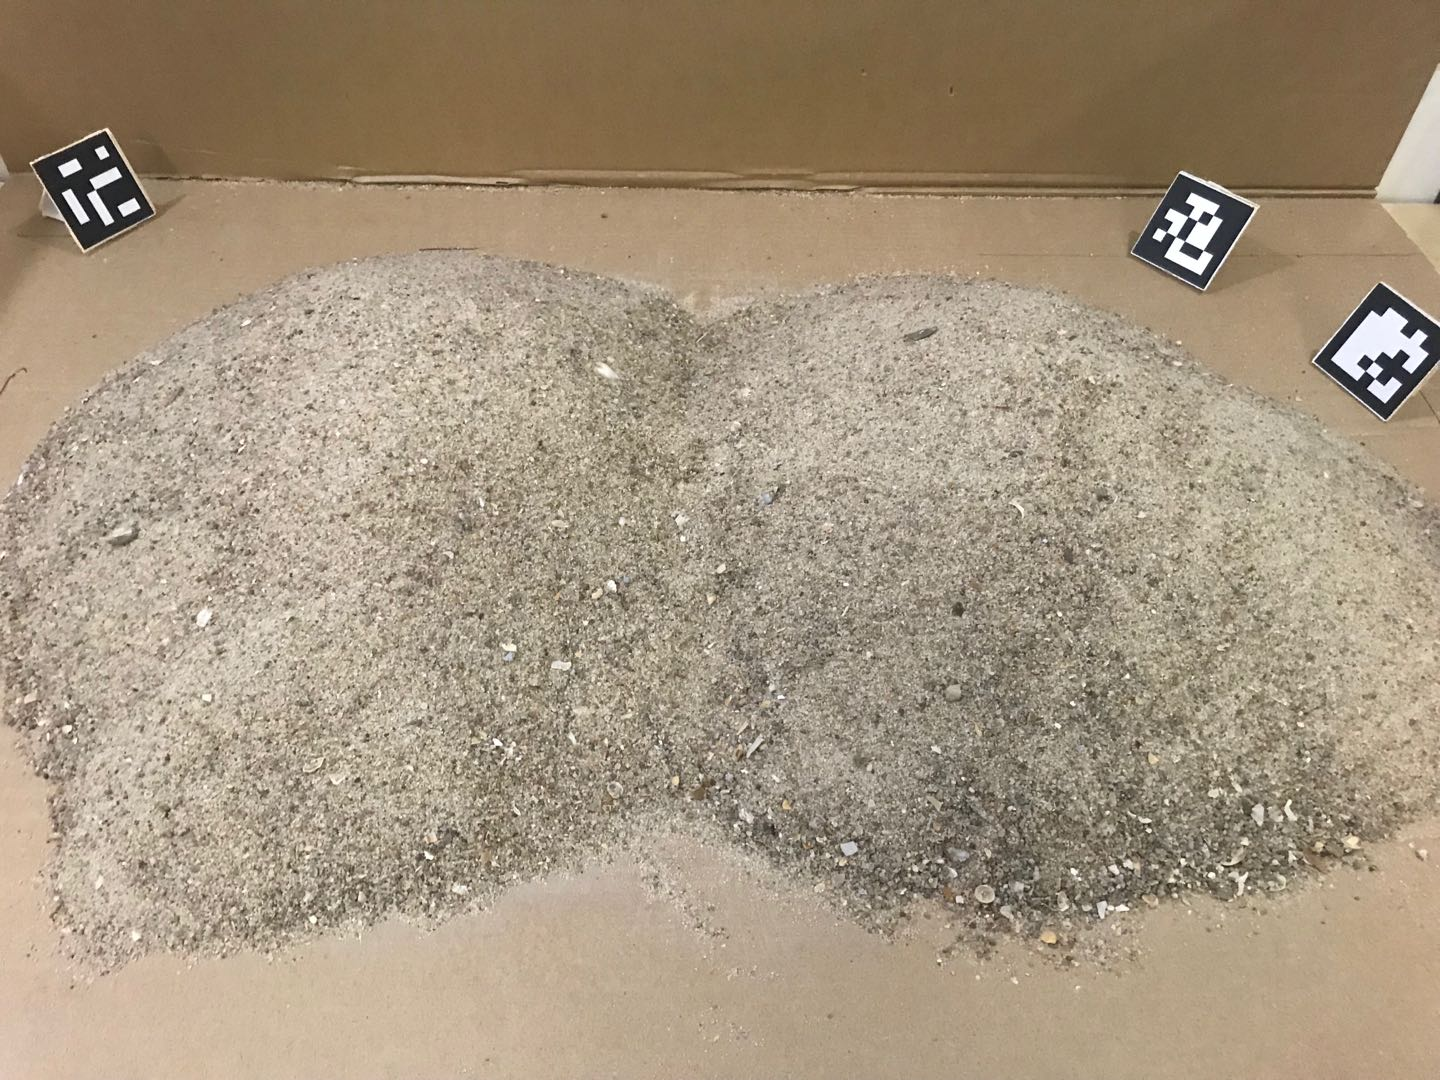
\includegraphics[width=7.5cm, height=5cm]{test_2.png} & 960*455\\
  3 & 215   & 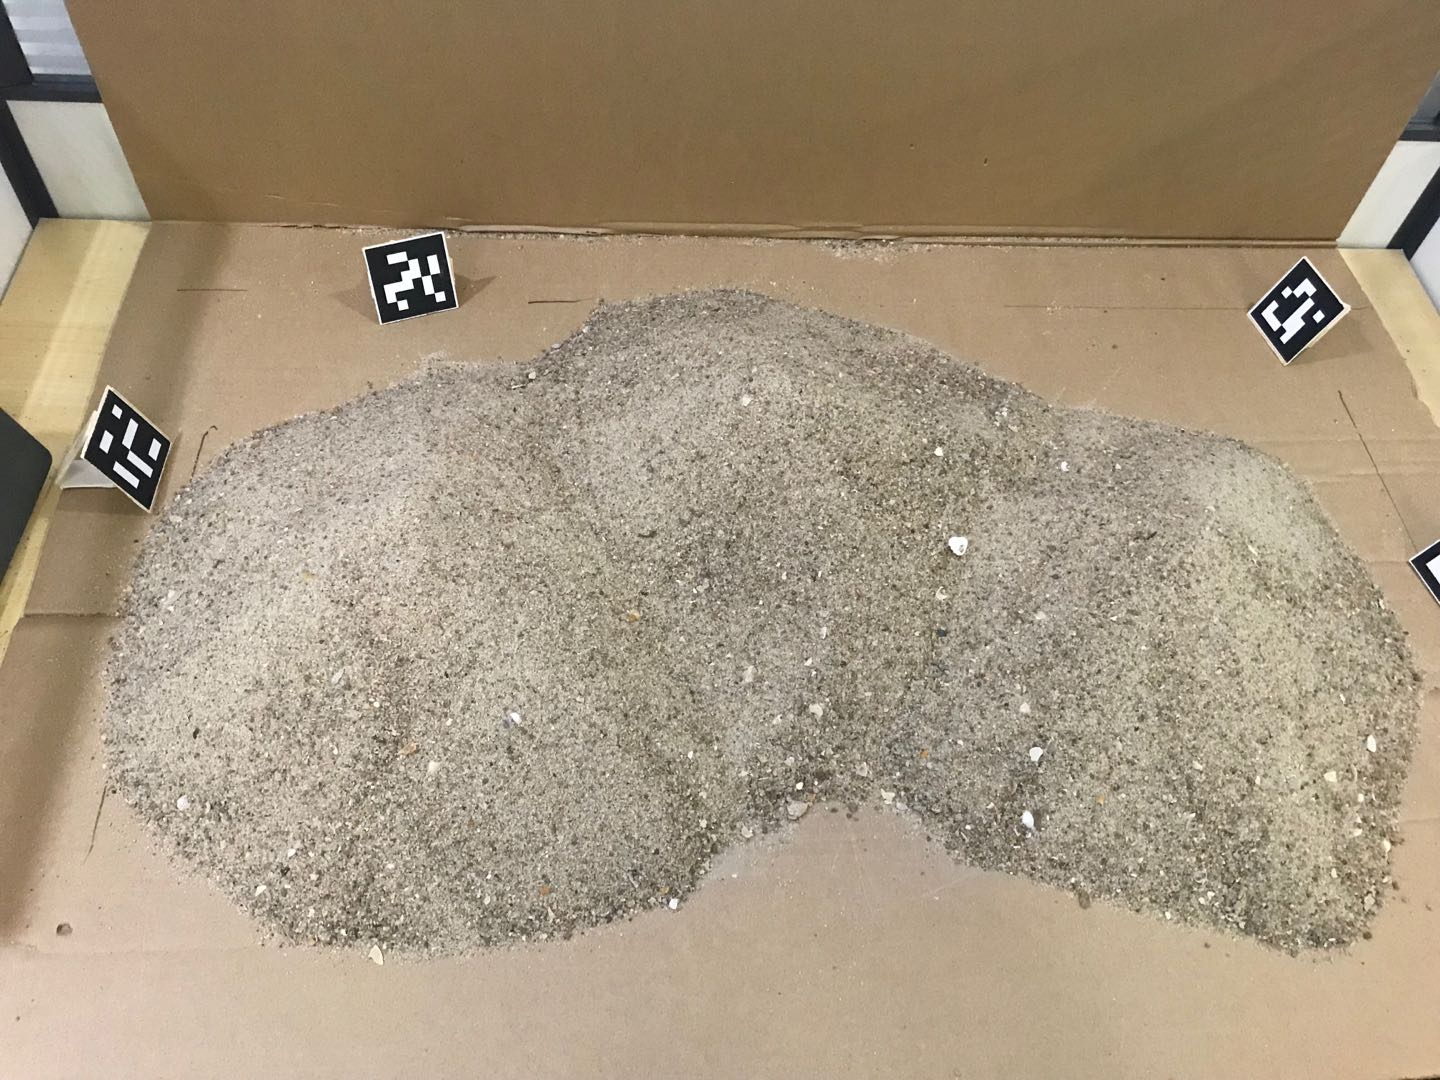
\includegraphics[width=7.5cm, height=5cm]{test_3.png} & 960*455\\
  \bottomrule
  \end{tabular}
\end{table}

\begin{table}[htb]
  \centering
  \caption{体积测量结果-\uppercase\expandafter{\romannumeral2}}
  \label{tab:volume_test_2}
  \begin{tabular}{C{8cm}C{2.0cm}C{1.2cm}C{3.6cm}}
  \toprule
  \textbf{稀疏点云} & \textbf{点集个数} & \textbf{尺度K} & \textbf{误差}\\
  \midrule
  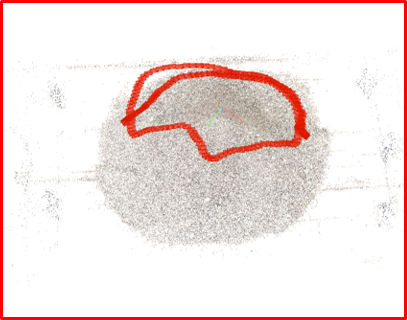
\includegraphics[width=7.5cm, height=5cm]{test_1_sparse.png}  &110149&1.945&-0.0259x-0.0331y-0.0873z+1=0\\
  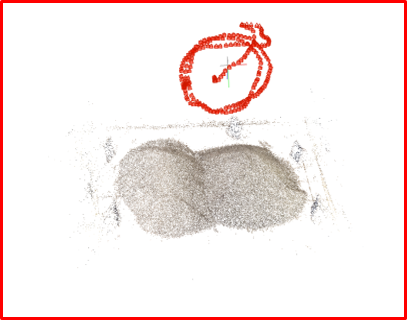
\includegraphics[width=7.5cm, height=5cm]{test_2_sparse.png}  & 86403&8.143& 0.0068x-0.0299y-0.0620z+1=0\\
  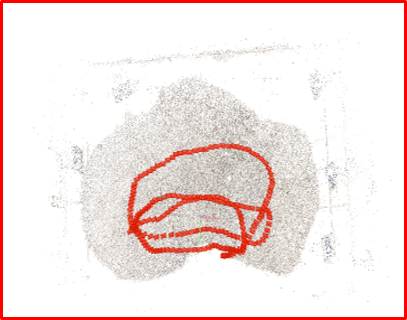
\includegraphics[width=7.5cm, height=5cm]{test_3_sparse.png}  & 83196&3.522& 0.0119x-0.0254y-0.0683z+1=0\\
  \bottomrule
  \end{tabular}
\end{table}


\begin{table}[htb]
  \centering
  \caption{体积测量结果-\uppercase\expandafter{\romannumeral3}}
  \label{tab:volume_test_3}
  \begin{tabular}{C{8cm}C{2.4cm}C{2.4cm}C{2.0cm}}
  \toprule
  \textbf{稠密点云} & \textbf{计算耗时(s)} & \textbf{堆体体积($cm^3$)} & \textbf{测量精度}\\
  \midrule
  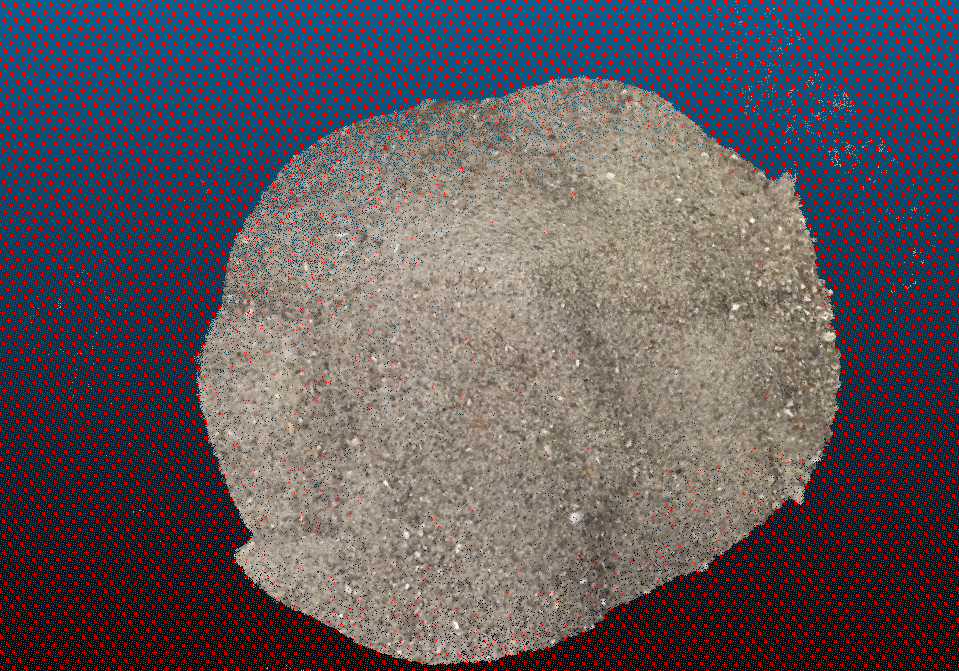
\includegraphics[width=7.5cm, height=5cm]{test_1_dense.png}  & 712 & 10340  &   1.1$\%$\\
  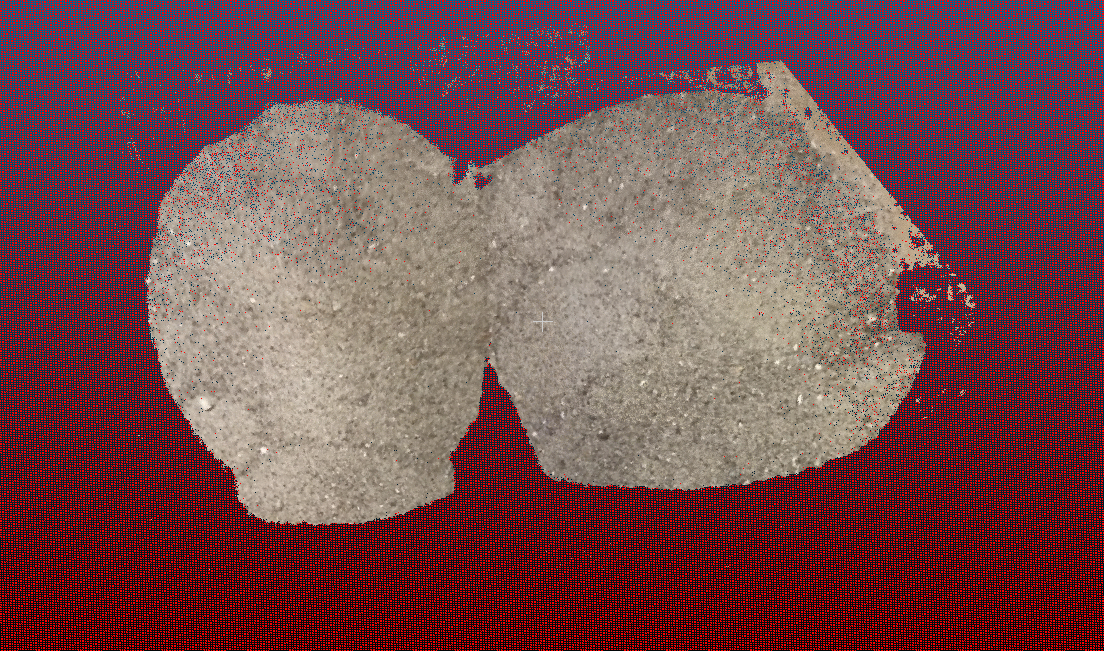
\includegraphics[width=7.5cm, height=5cm]{test_2_dense.png}  & 675 & 99032  &   0.9$\%$\\
  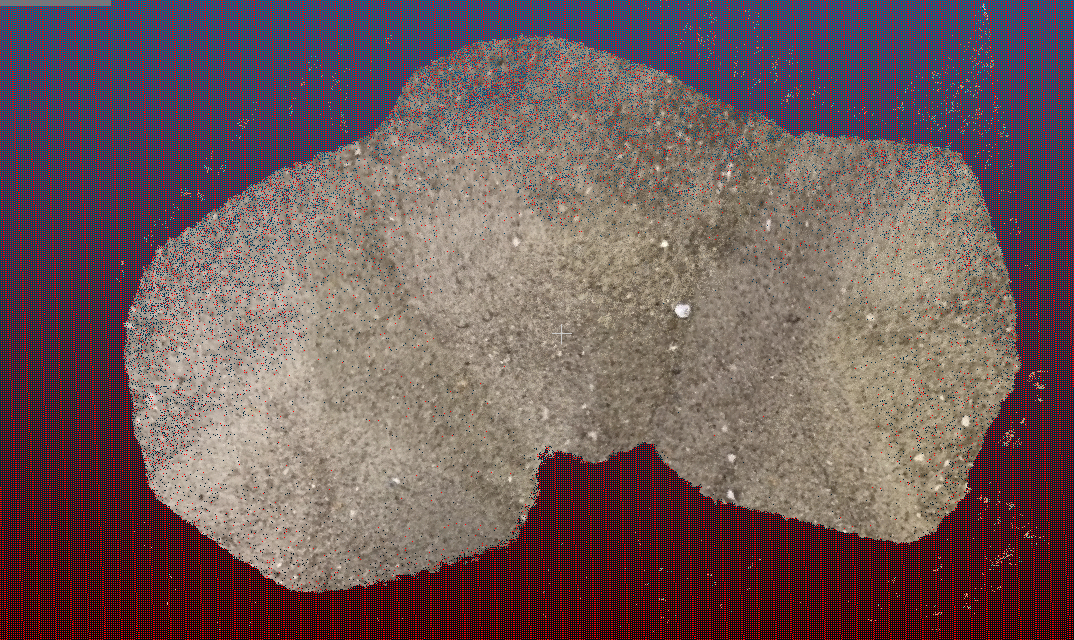
\includegraphics[width=7.5cm, height=5cm]{test_3_dense.png}  & 663 & 10552  &   1.3$\%$\\
  \bottomrule
  \end{tabular}
\end{table}


\section{本章小结}
本章分模块测试了无人机在非GPS场景下依靠纯视觉进行定位的效果与精度,以及改进后的三维重建的效果和基于纯视觉的堆体体积测量算法的准确度和稳定性。